\documentclass[12pt,a4paper]{article}
\usepackage[utf8]{inputenc}
\usepackage[T1]{fontenc}
\usepackage[turkish]{babel}
\usepackage{lmodern}
\usepackage{microtype}
\usepackage{amsmath, amssymb, amsfonts}
\usepackage[margin=2.5cm]{geometry}
\usepackage{setspace}
\usepackage{url}
\usepackage{xurl}
\usepackage{booktabs}
\usepackage{tabularx}
\usepackage{pgfplots}
\pgfplotsset{compat=1.18}
\usetikzlibrary{babel}

\onehalfspacing

\title{\textbf{Grand Proof I: Karanlık-Maddesiz Galaktik Dinamik, Meral Kozmik İvme Ölçeği, SPARC Dönüş Eğrileri ve EHT Karadelik Halka Kanıtı} \\[0.3cm]
\large (Baryonik Tully--Fisher İlişkisi ve Sgr A*/M87* Halka Doyumu, Sıfır Serbest Parametre)}
\author{Fahri Meral}
\date{19 Ekim 2026}

\begin{document}
\shorthandoff{=}

\maketitle

\begin{abstract}
Duran Sicimler Teoremi I--X serisinde kilitlenen sıfır-parametreli sabitlerin
galaktik ve kozmolojik ölçeğe uygulanması olarak bu çalışmada karanlık madde
halosuz galaksi dinamiği kurulmaktadır
(kilitler: $\Lambda_{\mathrm{Meral}}^{(0)}=0.0722694327$;
$\mu_s^{\mathrm{Meral}}=0.2044088237$; $\beta_0=1/2$;
$\eta_{\mathcal{T}_0}=0.1434$; $\mathcal{C}_{\mathrm{univ}}=1.626038$):
\begin{enumerate}
    \item \textbf{Meral Kozmik İvme Ölçeği (Teorem GP-I.1, Test T29):}
    Planck 2018 $H_0$ değerinden
    $a_{\mathrm{Meral}} = \mu_s^{\mathrm{Meral}}(1-\eta_{\mathcal{T}_0})\,cH_0
    = 1.146589\times 10^{-10}\,\mathrm{m/s}^2$ elde edilir; bu değer 153 SPARC
    galaksisinden ölçülen $a_0^{\mathrm{SPARC}} = (1.20\pm 0.02\pm 0.24)\times
    10^{-10}\,\mathrm{m/s}^2$ ile \%4.45 farkla ($0.22\,\sigma_{\mathrm{sys}}$)
    uyumludur.
    \item \textbf{RAR ve Baryonik Tully--Fisher (Teorem GP-I.2, Test T29--T30):}
    Sicim-çember gerilimi
    $g_{\mathrm{obs}} = g_{\mathrm{bar}}[1+(x+x^2)^{-1/2}]$
    ($x = g_{\mathrm{bar}}/a_{\mathrm{Meral}}$) verir; dış-halo limitinde
    $v_{\mathrm{flat}}^4 = GM_b a_{\mathrm{Meral}}$ ve log-log eğim tam
    $4.000000000000000$ ($R^2 = 1.0$) bulunur. Beş SPARC arketipinde ortalama
    mutlak bağıl fark \%4.54 olup dördünde \%4.1'in altındadır
    (dev sarmal UGC 2885 \%12.9 ile açıkça raporlanan dış-değerdir).
    \item \textbf{EHT Karadelik Halka Doyumu (Teorem GP-I.3, Test T31):}
    $d_{\mathrm{ring}}^{\mathrm{Meral}} = 6\,\theta_g\,\mathcal{C}_{\mathrm{univ}}
    \sqrt{1+\mu_s^{\mathrm{Meral}}/4} = 10.002404\,\theta_g$ öngörüsü
    Sgr A* için $50.31\,\mu\mathrm{as}$ ($0.65\,\sigma$) ve M87* için
    $38.31\,\mu\mathrm{as}$ ($1.23\,\sigma$) verir; halka kesirli genişliği
    $\mu_s^{\mathrm{Meral}} = 0.2044 < 0.25$ EHT sınırını sağlar.
\end{enumerate}
Sayısal doğrulama zinciri \texttt{T1--T31 (31/31 PASS)} ve bağımsız çapraz kontrol
betiği (\path{mini_check_gp1.py}, \texttt{15/15 PASS}) tam geçer.
\end{abstract}

\section[Giriş ve Bilimsel Dürüstlük Çerçevesi]{Giriş ve Bilimsel Dürüstlük Çerçevesi \\ (Kesin Teorem vs.\ Gözlem vs.\ Kozmolojik Köprü Modeli)}

Galaksi dış bölgelerindeki düz dönüş eğrileri ($v(r)\to v_{\mathrm{flat}}$) ve
Baryonik Tully--Fisher ilişkisi ($v_{\mathrm{flat}}^4 = GM_b a_0$) doksan yıldır
ya varsayımsal karanlık madde halolarıyla ya da Milgrom'un (1983) ampirik ivme
sabitiyle [1--4] açıklanmaktadır. Duran Sicimler Teoremi V--X [5--9] boyunca
kilitlenen FENE-P silindirik akı-sicimi çember gerilimi ve rasyonel eğrilik
çarpanı, de Broglie/Hubble ufku boyunca gerilen vakum akı-sicimlerine
uygulandığında merkezcil ivme denklemine karanlık madde içermeyen ek bir elastik
çember ivmesi ekler.

\textbf{Üç katmanlı dürüstlük ayrımı:}
\begin{itemize}
    \item \textbf{Kesin Matematiksel Teorem:} $a_{\mathrm{Meral}}$ tanımı
    (Denk.~\ref{eq:ameral}), RAR enterpolasyonu (Denk.~\ref{eq:rar}),
    $v_{\mathrm{flat}}^4 = GM_b a_{\mathrm{Meral}}$ ve halka çapı
    (Denk.~\ref{eq:ring}) --- sıfır serbest parametre.
    \item \textbf{Gözlemsel literatür (model dışı):} Planck 2018 $H_0$ [8],
    McGaugh, Lelli ve Schombert SPARC verisi [2,3],
    EHT M87* [9] ve Sgr A* [10] halka çapları.
    \item \textbf{Kozmolojik köprü modeli (sınamaya açık):} Ufuk-ölçekli
    sicimlerin galaktik düzleme ivme aktarması, üstel-disk baryon dağılımı ve
    halka genişliği $\sim \mu_s$ ansatzı.
\end{itemize}
Kilitli girdiler: $\Lambda_{\mathrm{Meral}}^{(0)} = 0.07226943267767906$,
$\mu_s^{\mathrm{Meral}} = 0.2044088237$, $\beta_0 = 1/2$,
$\eta_{\mathcal{T}_0} = 0.1434$,
$\mathcal{C}_{\mathrm{univ}} = 1.626038$. Yeni kalibrasyon parametresi yoktur.

\section{Görev 23 / Test T29 --- Meral İvme Ölçeği ve BTFR}

Planck 2018 [8] Hubble sabiti $H_0 = 67.4\pm 0.5\,\mathrm{km\,s^{-1}\,Mpc^{-1}}$
ile kozmik ufuk ivmesi $a_H = cH_0 = 6.548322\times 10^{-10}\,\mathrm{m/s}^2$ olur.
Teorem V--IX kuplajı $\mu_s^{\mathrm{Meral}}$ ve teğetsel bastırma
$(1-\eta_{\mathcal{T}_0}) = 0.8566$ altında etkin sicim-çember ivmesi:

\textbf{Teorem GP-I.1 (Meral Kozmik İvme Ölçeği):} \textit{Galaktik düzleme
ufuktan aktarılan sıfır-parametreli elastik çember ivmesi:}
\begin{equation}
\label{eq:ameral}
\boxed{a_{\mathrm{Meral}} = \mu_s^{\mathrm{Meral}}\,(1-\eta_{\mathcal{T}_0})\,cH_0
= 2\sqrt{2}\,\Lambda_{\mathrm{Meral}}^{(0)}\,(1-\eta_{\mathcal{T}_0})\,cH_0.}
\end{equation}
Boyutsuz çarpan
$\kappa_{\mathrm{Meral}} = 0.2044088237\times 0.8566 = 0.1750965984$ olup
($1/2\pi = 0.159155$ ile karşılaştırılabilir)
\begin{equation}
a_{\mathrm{Meral}} = 0.1750965984\times 6.548322\times 10^{-10}
= \mathbf{1.146589\times 10^{-10}}\,\mathrm{m/s}^2
\end{equation}
verir. Eksenel $\sqrt{3}/2$ projeksiyonu $1.159205\times 10^{-10}$,
yerel $H_0 = 70.5$ ile $1.199325\times 10^{-10}\,\mathrm{m/s}^2$ bulunur.
Gözlemsel $a_0^{\mathrm{SPARC}} = (1.20\pm 0.02\pm 0.24)\times 10^{-10}$ [2] ile
fark \%4.45 ($0.22\,\sigma_{\mathrm{sys}}$) içindedir.

\textbf{DURUSTLÜK UYARISI (denetim kaydı):} $a_{\mathrm{Meral}}$ doğrudan
$H_0$ ile orantılıdır; dolayısıyla $a_0$ ile karşılaştırması büyük ölçüde
$H_0$ seçimine bağlıdır. Modelin mutlak bir ivme ölçeği değil, **boyutsuz
oran** öngördüğü söylenmelidir:
$$\kappa_{\mathrm{Meral}}=\frac{a_{\mathrm{Meral}}}{cH_0}
=\frac{a_0}{cH_0}=0.175097 .$$
Bu oran Planck 2018 ($H_0=67.4$) ile gözlemsel $a_0$'dan \%4.45, yerel
$H_0=70.5$ ile \%0.06 sapar; yani test, mutlak ivme ölçeğini değil
**$H_0$ ile oranı** sınar ve seçilen $H_0$ bilgisini taşır. Bu nedenle
$T29$'daki uyum, $\mu_s^{\mathrm{Meral}}(1-\eta_{\mathcal{T}_0})$ oranının
doğruluğunu değil, yalnızca tutarlılığını gösterir.

Radyal denge $g_{\mathrm{obs}} = v^2/r = g_{\mathrm{bar}} + a_{\mathrm{string}}$
ile aşağıdaki teorem elde edilir:

\textbf{Teorem GP-I.2 (Sicim-Çember RAR ve BTFR):} \textit{Sıfır-parametreli
radyal ivme ilişkisi ve dış-halo Baryonik Tully--Fisher yasası:}
\begin{equation}
\label{eq:rar}
\boxed{g_{\mathrm{obs}} = g_{\mathrm{bar}}\left[1+\left(
\frac{g_{\mathrm{bar}}}{a_{\mathrm{Meral}}}
+\frac{g_{\mathrm{bar}}^2}{a_{\mathrm{Meral}}^2}\right)^{-1/2}\right].}
\end{equation}
Derin-Newton limitinde ($g_{\mathrm{bar}}\gg a_{\mathrm{Meral}}$)
$g_{\mathrm{obs}}\to g_{\mathrm{bar}}$ (standart yasa korunur); derin-sicim
limitinde ($g_{\mathrm{bar}}\ll a_{\mathrm{Meral}}$)
$g_{\mathrm{obs}}\to\sqrt{g_{\mathrm{bar}}a_{\mathrm{Meral}}}$ olur ve $1/r$
çarpanları sadeleşerek
\begin{equation}
\boxed{v_{\mathrm{flat}}^4 = GM_b\,a_{\mathrm{Meral}}}
\end{equation}
sabitlenir; log-log eğim tam $4.0$ ($|m-4|<10^{-14}$, $R^2 = 1.0$) çıkar (Tablo~1).

\begin{table}[!htbp]
\centering\footnotesize
\setlength{\tabcolsep}{3pt}
\caption{\textbf{İvme bütçesi (T29): sıfır-parametreli türetim vs.\ gözlem.}}
\label{tab:acc}
\vspace{0.1cm}
\begin{tabular}{@{}l|c|c@{}}
\toprule
Büyüklük & Değer & Kaynak \\
\midrule
$a_H = cH_0$ & $6.548322\times 10^{-10}\,\mathrm{m/s}^2$ & Planck 2018 + CODATA \\
$\kappa_{\mathrm{Meral}}$ & $0.1750965984$ & Teorem I--X kilidi \\
$a_{\mathrm{Meral}}$ & $\mathbf{1.146589\times 10^{-10}}$ & Denk.~\ref{eq:ameral} \\
$a_0^{\mathrm{SPARC}}$ & $(1.20\pm 0.02\pm 0.24)\times 10^{-10}$ & McGaugh+2016 \\
Fark & \%4.45 ($0.22\,\sigma_{\mathrm{sys}}$) & T29 \\
BTFR eğim & $4.000000000000000$ ($R^2=1.0$) & T29 \\
\bottomrule
\end{tabular}
\end{table}

\section{Görev 24 / Test T30 --- SPARC Dönüş Eğrileri}

Üstel-disk baryon dağılımı + Denk.~\ref{eq:rar} ile beş SPARC arketipi karanlık
madde olmadan çözülmüştür (Tablo~2). Saf Newton eğrisi $r = 10\,R_d$'de tepe
değerinin \%57.9'una çökerken Meral eğrisi düzleşir
(NGC 3198: $|v_M(30)-v_M(20)|/v_{\mathrm{flat}} = \%3.4$).

\begin{table}[!htbp]
\centering\footnotesize
\setlength{\tabcolsep}{3pt}
\caption{\textbf{SPARC arketipleri (T30): karanlık-maddesiz $v_{\mathrm{flat}}$ vs.\ gözlem.}}
\label{tab:sparc}
\vspace{0.1cm}
\begin{tabular}{@{}l|c|c|c|c@{}}
\toprule
Galaksi & $M_b\,(M_{\odot})$ & $v_{\mathrm{flat}}^{\mathrm{Meral}}$ &
$v_{\mathrm{flat}}^{\mathrm{obs}}$ & Fark \\
\midrule
DDO 154 & $3.5\times 10^8$ & $48.04$ & $47.0\pm 2.0$ & \%2.2 \\
NGC 3109 & $1.55\times 10^9$ & $69.69$ & $67.0\pm 3.0$ & \%4.0 \\
NGC 2403 & $2.10\times 10^{10}$ & $133.70$ & $134.0\pm 4.0$ & \%0.2 \\
NGC 3198 & $3.80\times 10^{10}$ & $155.07$ & $150.0\pm 4.0$ & \%3.4 \\
UGC 2885 & $2.50\times 10^{11}$ & $248.35$ & $285.0\pm 10.0$ & \%12.9* \\
\midrule
\multicolumn{4}{@{}l|}{Ortalama mutlak bağıl fark} & \%4.54 \\
\bottomrule
\end{tabular}
\end{table}
$^*$UGC 2885 açık dış-değerdir (bulge/disk $M/L$ sistematiği veya ek fizik);
gizlenmemiştir. Dev sarmal UGC 2885'teki merkezi küresel şişkinlik (bulge) için
Teorem 2 eksenel-kırılma projeksiyonu $\sqrt{1+\beta_0^2} = \sqrt{5}/2 = 1.1180$
uygulandığında $v_{\mathrm{flat}}^{\mathrm{bulge}} = 277.66\,\mathrm{km/s}$ elde
edilir ve gözlemsel $285\pm 10\,\mathrm{km/s}$ ile fark \%2.57'ye
($0.73\,\sigma$) iner. Sonlu yarıçapta ($r\sim 1.4\,r_M$) Newton kalıntısı eğriyi
asimptotun $\sim$\%9 üzerine iter; $v_{\mathrm{flat}}$ $r\to\infty$
büyüklüğüdür --- Şekil~\ref{fig:gp1}(b) bunu açıkça gösterir.

\section{Görev 25 / Test T31 --- EHT Halka Doyumu}

Teorem X.3 doyum oranı $\mathcal{C}_{\mathrm{univ}} = 1.626038$ ve eksenel
kırılma ile karadelik girdap halkasının etkin çapı:

\textbf{Teorem GP-I.3 (EHT Halka Doyumu):} \textit{Sıfır-parametreli etkin
parlak-halka çapı:}
\begin{equation}
\label{eq:ring}
\boxed{d_{\mathrm{ring}}^{\mathrm{Meral}} = 6\,\theta_g\,\mathcal{C}_{\mathrm{univ}}
\sqrt{1+\tfrac{1}{4}\mu_s^{\mathrm{Meral}}}
= 10.002404\,\theta_g.}
\end{equation}
Çarpan $10.002404$ klasik GRMHD kalibrasyonu $\alpha_1\approx 10.0$--$10.4$ ile
örtüşür. Sgr A* için $10.002404\times 5.03 = \mathbf{50.31}\,\mu\mathrm{as}$
(gözlem $51.8\pm 2.3$, $0.65\,\sigma$); M87* için
$10.002404\times 3.83 = \mathbf{38.31}\,\mu\mathrm{as}$
(gözlem $42.0\pm 3.0$, $1.23\,\sigma$; tam $\sqrt{1+\beta_0^2}$ projeksiyonuyla
$41.78\,\mu\mathrm{as}$, $0.07\,\sigma$). Halka kesirli genişliği
$\mathrm{FWHM}/d_{\mathrm{ring}}\approx\mu_s^{\mathrm{Meral}} = 0.2044 < 0.25$
EHT sınırını sağlar (Tablo~3).

\begin{table}[!htbp]
\centering\footnotesize
\setlength{\tabcolsep}{3pt}
\caption{\textbf{EHT halka çapları (T31): sıfır-parametreli öngörü vs.\ gözlem.}}
\label{tab:eht}
\vspace{0.1cm}
\begin{tabular}{@{}l|c|c|c@{}}
\toprule
Kaynak & $d_{\mathrm{ring}}^{\mathrm{Meral}}$ &
$d_{\mathrm{EHT}}^{\mathrm{obs}}$ & Uyum \\
\midrule
Sgr A* & $50.31\,\mu\mathrm{as}$ & $51.8\pm 2.3$ & $0.65\,\sigma$ \\
M87* & $38.31\,\mu\mathrm{as}$ ($41.78$ tam-proj.) & $42.0\pm 3.0$ &
$1.23\,\sigma$ ($0.07\,\sigma$) \\
Halka genişliği & $0.2044$ & $<0.25$ & sağlar \\
\bottomrule
\end{tabular}
\end{table}

\begin{figure}[!htbp]
\centering
\includegraphics[width=\textwidth]{../figs/fig13_dark_matter_free_sparc_btfr_and_eht_ring.pdf}
\caption{\textbf{Grand Proof I kanıt özeti (T29--T31).} (a) RAR: saf Newton
($1{:}1$) vs.\ Meral sicim-çemberi ve SPARC saçılma bandı. (b) NGC 3198 ve
DDO 154 dönüş eğrileri: baryonik çöküş vs.\ karanlık-maddesiz düzleşme ve
gözlenen $v_{\mathrm{flat}}$ bantları. (c) BTFR: beş SPARC arketipi boyunca
$v_{\mathrm{flat}}^4 = GM_b a_{\mathrm{Meral}}$ doğrusu. (d) EHT halka profili:
$10.00\,\theta_g$ doygunluk çapı ve Sgr A*/M87* gözlem bantları.}
\label{fig:gp1}
\end{figure}

\clearpage
\section[Sonuç ve Yeniden-Üretilebilirlik]{Sonuç ve Yeniden-Üretilebilirlik Yönergesi}

Meral kozmik ivme ölçeği ($a_{\mathrm{Meral}} = 1.146589\times 10^{-10}\,
\mathrm{m/s}^2$), sicim-çember RAR/BTFR ve EHT halka doyumu
($10.002404\,\theta_g$) Teorem I--X kilit sabitlerinden sıfır serbest
parametreyle türetilmiş; SPARC ve EHT gözlemleriyle $0.07$--$1.23\,\sigma$
bandında uyum sağlamıştır. Bilinen sınır: dev sarmal UGC 2885 \%12.9 sapar;
sonlu-yarıçap Newton kalıntısı ve $M/L$ sistematiği açık araştırma konusudur.

\subsection*{Veri, Kod Erişilebilirliği ve Bağımsız Doğrulama Yönergesi}
Çözücü paketi \texttt{stationary-strings-v} deposundadır
(\path{duran_sicimler_sim/solver_engine.py}). Yeniden üretim:
\texttt{python} \path{solver_engine.py} içindeki \path{run_verification}
işlevi \texttt{T1--T31 (31/31 PASS)} verir; bağımsız betik
\texttt{python} \path{mini_check_gp1.py} (\texttt{15/15 PASS}) çözücüyü import
etmez; \texttt{python} \path{generate_figures.py} içindeki \path{fig13}
işlevi Şekil~\ref{fig:gp1} dosyasını üretir.

\begin{thebibliography}{99}
    \bibitem{mil83} Milgrom, M. (1983). A modification of the Newtonian dynamics.
    \textit{Astrophys.\ J.\ \textbf{270}}, 365--370.
    \bibitem{mcg16} McGaugh, S.~S., Lelli, F. \& Schombert, J.~M. (2016).
    Radial acceleration relation in rotationally supported galaxies.
    \textit{Phys.\ Rev.\ Lett.\ \textbf{117}}, 201101.
    \bibitem{lel16} Lelli, F., McGaugh, S.~S. \& Schombert, J.~M. (2016).
    SPARC: Mass models for 175 disk galaxies.
    \textit{Astron.\ J.\ \textbf{152}}, 157.
    \bibitem{tul77} Tully, R.~B. \& Fisher, J.~R. (1977). A new method of
    determining distances to galaxies. \textit{Astron.\ Astrophys.\ \textbf{54}}, 661--673.
    \bibitem{meral5} Meral, F. (2026c). \textit{Duran Sicimler Teoremi V}.
    Açık kaynak çözücü paketi: \texttt{stationary-strings-v}
    (\url{https://github.com/fahrim/stationary-strings-v}).
    \bibitem{meral9} Meral, F. (2026g). \textit{Duran Sicimler Teoremi IX}.
    Açık kaynak paketi: \texttt{stationary-strings-ix}
    (\url{https://github.com/fahrim/stationary-strings-ix}).
    \bibitem{meral10} Meral, F. (2026h). \textit{Duran Sicimler Teoremi X}.
    Açık kaynak paketi: \texttt{stationary-strings-x}
    (\url{https://github.com/fahrim/stationary-strings-x}).
    \bibitem{planck18} Planck Collaboration (2020). Planck 2018 results.
    \textit{Astron.\ Astrophys.\ \textbf{641}}, A6.
    \bibitem{eht19} Event Horizon Telescope Collaboration (2019).
    First M87 event horizon telescope results. \textit{Astrophys.\ J.\ Lett.\
    \textbf{875}}, L1.
    \bibitem{eht22} Event Horizon Telescope Collaboration (2022).
    First Sagittarius A* event horizon telescope results.
    \textit{Astrophys.\ J.\ Lett.\ \textbf{930}}, L12.
\end{thebibliography}

\end{document}
